% !TeX encoding = UTF-8
% !TeX spellcheck = pl_PL

% $Id:$

%Author: Wojciech Domski
%Szablon do ząłożeń projektowych, raportu i dokumentacji z steorwników robotów
%Wersja v.1.0.0
%


%% Konfiguracja:
\newcommand{\kurs}{Roboty Mobilne}
\newcommand{\formakursu}{Projekt}

%odkomentuj właściwy typ projektu, a pozostałe zostaw zakomentowane
\newcommand{\doctype}{Za\l{}o\.{z}enia projektowe} %etap I
%\newcommand{\doctype}{Raport} %etap II
%\newcommand{\doctype}{Dokumentacja} %etap III

%wpisz nazwę projektu
\newcommand{\projectname}{Robot mobilny z platformą fotowoltaniczną}

%wpisz akronim projektu
%\newcommand{\acronim}{WK}

%wpisz Imię i nazwisko oraz numer albumu
\newcommand{\osobaA}{Paula \textsc{Langkafel}, 235373}
%w przypadku projektu jednoosobowego usuń zawartość nowej komendy
\newcommand{\osobaB}{Albert \textsc{Lis}, 235534}

\newcommand{\osobaC}{Michał \textsc{Moruń}, 235986}

%wpisz termin w formie, jak poniżej dzień, parzystość, godzina
\newcommand{\termin}{wtorek TP 17}

%wpisz imię i nazwisko prowadzącego
\newcommand{\prowadzacy}{mgr in\.{z}. Michał \textsc{Błędowski}}

\documentclass[10pt, a4paper]{article}

%Preambuła dokumentu

% linki w spisie tresci, bibliografi
\usepackage[bookmarks=true,bookmarksnumbered=false,unicode=true,pdftex=true, colorlinks,filecolor=black,linkcolor=black,urlcolor=black,citecolor=black]{hyperref}

%ustawienie rozmiaru papieru
\usepackage[a4paper, left=2.5cm, right=2.5cm, top=2.5cm, bottom=2.5cm, headsep=1.2cm]{geometry}

%rozmaite ustawienia pozwalające okreslić język

%NALEŻY wybrać jeden z pakietów
%\usepackage{polski} %przydatne podczas składania dokumentów w j. polskim
\usepackage[polish]{babel}  % pakiet lokalizujący dokument w języku polskim
%\usepackage[british]{babel}

\usepackage{indentfirst}	% polski styl pisania (np. rozpoczecie pierwszego akapitu
% pod nazwa rozdzialu od wciecia)
%\usepackage[OT4]{fontenc}
\usepackage[utf8]{inputenc} % w miejsce utf8 można wpisać latin2 bądź cp1250,
% w zależności od tego w jaki sposób kodowane są 
% polskie znaki diakrytyczne przy wprowadzaniu 
% z klawiatury.
%kodowanie znaków, zależne od systemu
\usepackage[T1]{fontenc} %poprawne składanie polskich czcionek

%OPEROWANIE NA OBRAZACH
\usepackage{graphicx}       % pakiet graficzny, umożliwiający m.in.
% import grafik w formacie eps
%\usepackage{epstopdf}		% pozwala na importowanie grafik w formacie eps
% przy użyciu pdflatex
\usepackage[update,prepend]{epstopdf}
\usepackage{rotating}       % pakiet umożliwiający obracanie rysunków
\usepackage{subfigure}      % pakiet umożliwiający tworzenie podrysunków
\usepackage{epic}           % pakiet umożliwiający rysowanie w środowisku latex
\usepackage{psfrag}         % pakiet umożliwiający podmianę łańcuchów znaków 
% w plikach eps
%\usepackage{curves}         % pakiet do wykreslania krzywych

%pakiety dodające dużo dodatkowych poleceń matematycznych
\usepackage{amsfonts}       % pakiet z rozmaitymi czcionkami matematycznymi
%\usepackage{amssymb}        % pakiet z rozmaitymi symbolami matematycznymi
\usepackage{amsmath}        % pakiet z rozmaitymi środowiskami matematycznymi

\usepackage{fp}             % pakiet z funkcjami operujacymi 
% na liczbach zmiennoprzecinkowych
\usepackage{calc}           % pakiet umożliwiający operacje arytmetyczne
% na tzw. licznikach (liczbach całkowitych)
\usepackage{leftidx}		% indeksy górne i dolne po lewej stronie

%definicje matematyczne
\providecommand{\abs}[1]{\lvert#1\rvert}
\providecommand{\norm}[1]{\lVert#1\rVert}

%pakiety wspomagające i poprawiające składanie tabel
\usepackage{supertabular}
\usepackage{array}
\usepackage{tabularx}
\usepackage{hhline}
\usepackage{longtable}		% wsparcie dla dlugich tabel
\usepackage{multicol}		% podzial strony na wiele kolumn

%pakiet do BibTex
\usepackage{cite}

\usepackage{url} %pakiet pozawalający na dodawanie adresów url w bibliografi

%pakiet wypisujący na marginesie etykiety równań i rysunków zdefiniowanych przez \label{}, chcąc wygenerować finalną wersję dokumentu wystarczy usunąć poniższą linię
%\usepackage{showlabels}

\usepackage{float}			% lepsza obsluga mechanizmow obiektow plywajacych
% wymuszenie wstawienia np. tabeli, obrazka w danym miejscu przez [H]

\usepackage{listings}       % pakiet dedykowany zrodlom programow
\usepackage{color}


\definecolor{dkgreen}{rgb}{0,0.6,0}
\definecolor{gray}{rgb}{0.5,0.5,0.5}
\definecolor{mauve}{rgb}{0.58,0,0.82}

\lstset{ %
	language=C,                % the language of the code
	basicstyle=\small,           % the size of the fonts that are used for the code
	numbers=left,                   % where to put the line-numbers
	numberstyle=\footnotesize\color{gray},  % the style that is used for the line-numbers
	stepnumber=1,                   % the step between two line-numbers. If it's 1, each line 
	% will be numbered
	numbersep=5pt,                  % how far the line-numbers are from the code
	backgroundcolor=\color{white},      % choose the background color. You must add \usepackage{color}
	showspaces=false,               % show spaces adding particular underscores
	showstringspaces=false,         % underline spaces within strings
	showtabs=false,                 % show tabs within strings adding particular underscores
	%frame=single,                   % adds a frame around the code
	rulecolor=\color{black},        % if not set, the frame-color may be changed on line-breaks within not-black text (e.g. comments (green here))
	tabsize=2,                      % sets default tabsize to 2 spaces
	captionpos=b,                   % sets the caption-position to bottom
	breaklines=true,                % sets automatic line breaking
	breakatwhitespace=false,        % sets if automatic breaks should only happen at whitespace
	%title=\lstname,                   % show the filename of files included with \lstinputlisting;
	% also try caption instead of title
	keywordstyle=\color{blue},          % keyword style
	commentstyle=\color{dkgreen},       % comment style
	stringstyle=\color{mauve},         % string literal style
	escapeinside={\%*}{*)},            % if you want to add LaTeX within your code
	morekeywords={*,...},              % if you want to add more keywords to the set
	deletekeywords={...}              % if you want to delete keywords from the given language
}

%polish signs in lst code
\lstset{literate=%
	{ą}{{\k{a}}}1
	{ć}{{\'c}}1
	{ę}{{\k{e}}}1
	{ł}{{\l}}1
	{ń}{{\'n}}1
	{ó}{{\'o}}1
	{ś}{{\'s}}1
	{ż}{{\.z}}1
	{ź}{{\'z}}1
	{Ą}{{\k{A}}}1
	{Ć}{{\'C}}1
	{Ę}{{\k{E}}}1
	{Ł}{{\L}}1
	{Ń}{{\'N}}1
	{Ó}{{\'O}}1
	{Ś}{{\'S}}1
	{Ż}{{\.Z}}1
	{Ź}{{\'Z}}1
}

\usepackage{verbatim}       % pakiet dedykowany rozmaitym wydrukom tekstowym
\usepackage{ifthen}         % pakiet umożliwiający tworzenie prostych programów
% (m.in. zawiera instrukcje powtórzeniowe 
% i warunkowe)
\usepackage{upquote}		%normal quotations marks ' and `

% deklaracje wymagane przez pakiet theorem automatycznie ladowany w przypadku
% klasy dokumentu article
%
\newtheorem{Dn}{Definicja}[section]     % deklaracja srodowiska definicja
\newtheorem{La}[Dn]{Lemat}                % deklaracja srodowiska lemat
\newtheorem{Tm}[Dn]{Twierdzenie}          % deklaracja srodowiska twierdzenie
\newtheorem{Rk}[Dn]{Spostrze{\.z}enie}  % deklaracja srodowiska spostrzezenie
\newtheorem{Am}[Dn]{Algorytm}           % deklaracja srodowiska algorytm
\newtheorem{As}[Dn]{Za{\l}o{\.z}enie}   % deklaracja srodowiska zalozenie
\newtheorem{Pn}[Dn]{Propozycja}           % deklaracja srodowiska propozycja
\newtheorem{Py}[Dn]{W{\l}asno{\'s}{\'c}}  % deklaracja srodowiska wlasnosc
\newtheorem{Cy}[Dn]{Wniosek}              % deklaracja srodowiska wniosek
\newtheorem{Ee}[Dn]{Przyk{\l}ad}        % deklaracja srodowiska przyklad
\newtheorem{Ex}{{\'C}wiczenie}          % deklaracja srodowiska cwiczenie

%helps to specify width of a column in table
%\begin{tabular}{|C{1cm}|c|c|c|c|c|c|c|c|c|c|}
%first column will have widht of 1cm
\newcolumntype{L}[1]{>{\raggedright\let\newline\\\arraybackslash\hspace{0pt}}m{#1}}
\newcolumntype{C}[1]{>{\centering\let\newline\\\arraybackslash\hspace{0pt}}m{#1}}
\newcolumntype{R}[1]{>{\raggedleft\let\newline\\\arraybackslash\hspace{0pt}}m{#1}}

\sloppy			%zawija bardzo długie linie

%\pagenumbering{gobble}% Remove page numbers (and reset to 1)
	
\begin{document}

\def\tablename{Tabela}	%zmienienie nazwy tabel z Tablica na Tabela

\begin{titlepage}
	\begin{center}
		\textsc{\LARGE \formakursu}\\[1cm]		
		\textsc{\Large \kurs}\\[0.5cm]		
		\rule{\textwidth}{0.08cm}\\[0.4cm]
		{\huge \bfseries \doctype}\\[1cm]
		{\huge \bfseries \projectname}\\[0.5cm]
%		{\huge \bfseries \acronim}\\[0.4cm]
		\rule{\textwidth}{0.08cm}\\[1cm]
		
		\begin{flushright} \large
		\emph{Skład grupy:}\\
		\osobaA\\
		\osobaB\\
		\osobaC\\[0.4cm]
		
		\emph{Termin: }\termin\\[0.4cm]

		\emph{Prowadzący:} \\
		\prowadzacy \\
		
		\end{flushright}
		
		\vfill
		
		{\large \today}
	\end{center}	
\end{titlepage}

\newpage
\tableofcontents
\newpage

%Obecne we wszystkich dokumentach
\section{Opis projektu}
Celem projektu jest stworzenie robota sterowanego który będzie zbierał informacje o natężeniu światła w danej okolicy. Robot powinien poruszać się na ograniczonej przestrzeni i cyklicznie przykładowo co 20cm pobierać informacje o natężeniu światła. Po zgromadzeniu danych robot zostanie podłączony do komputera za pomocą portu szeregowego i stamtąd zostaną pobrane dane do wizualizacji.

	\begin{figure}[H]
		\centering
		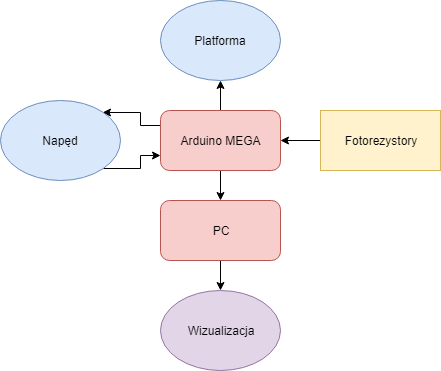
\includegraphics[width=0.7\textwidth]{diag3.png}
		\caption{Architektura robota}
		\label{fig:Architektura robota}
	\end{figure}

\section{Założenia projektowe}

\subsection{Mechanika}
\begin{enumerate}
	\item Sterowanie robotem
	\newline
	Skręcanie zostanie zrealizowane za pomocą serwa $180^\circ$ natomiast napęd za pomocą silnika szczotkowego DC.
	
	\item Sterowanie platformą
	\newline
	Realizowane w oparciu o serwomechanizmy $180^\circ$ oraz $360^\circ$. To pierwsze zapewni pozycjonowanie w  kierunku wertykalnym, a drugie w kierunku horyzontalnym. Zostanie również zastosowana przekładnia przy obrocie wokół własnej osi by uzyskać dokładniejsze oraz bardziej stabilne pozycjonowanie.
	
	\item Podstawa oraz separator fotorezystorów
	\newline
	Zbudowana z klocków lego. Posiada duże możliwości dopasowania do zmian w trakcie projektu.
	
\end{enumerate}

\subsection{Elektronika}
\begin{enumerate}
	\item Mikrokontroler
	\newline
	Do sterowania robotem zostanie użyty sterownik Arduino Mega2560.
	
	\item Zasilanie
	\newline
	Oparte o akumulatory li-ion 18650 lub powerbank. Ustalenie napięcia 5V za pomocą przetwornicy step-up MT3608 do zasilania płytki Arduino oraz napędu platformy i robota.
	
	\item Pozycjonowanie
	\newline
	Użyte zostaną 4 odseparowane fotorezystory gl5516. Ich wartości mierzone będą za pomocą portów analogowych  sterownika Arduino Mega2560.
	
	\item Pozycja
	\newline
	Do ustalania bieżącej pozycji zostaną wykorzystane enkodery SparkFun SEN-12617.
	
	\item Pomiar natężenia światła
	\newline
	Wykorzystany zostanie czujnik
\end{enumerate}

\section{Harmonogram pracy}

\subsection{Zakres prac}
\begin{enumerate}
	\item Zapoznanie się z mikrokontrolerem
	\newline
	Wykorzystane to tego celu zostaną poradniki ze strony www.forbot.pl.
\end{enumerate}
\subsection{Kamienie milowe}
\begin{enumerate}
	\item Zbudowanie robota
	\item Implementacja modułu elektronicznego do platformy
	\item Implementacja algorytmów sterowania platformą
\end{enumerate}

\subsection{Diagram Gantta}

	\begin{figure}[H]
		\centering
		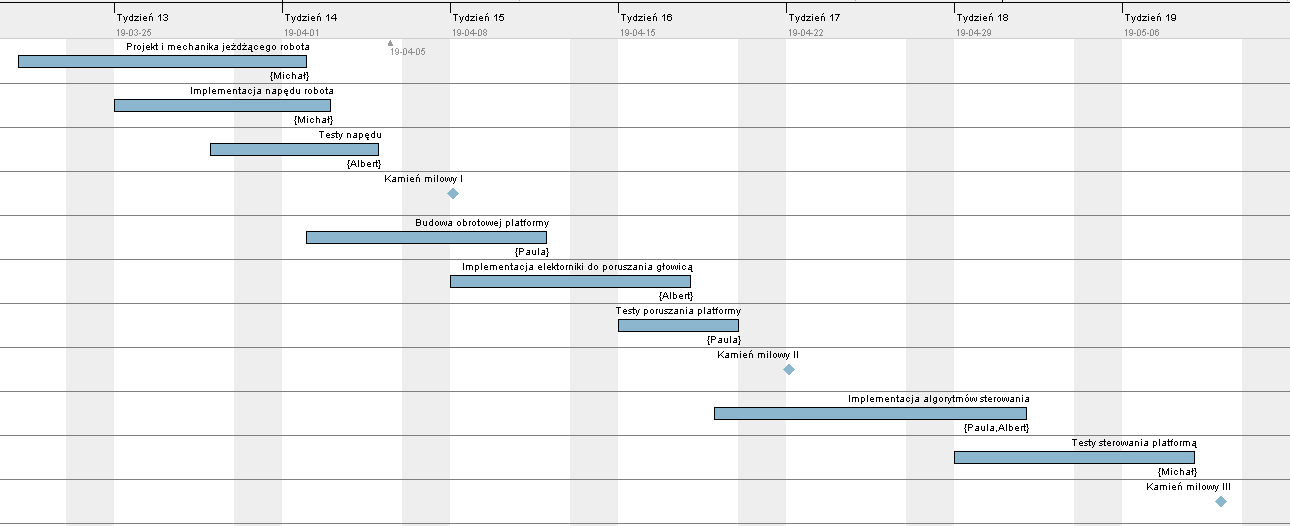
\includegraphics[width=1.1\textwidth]{gantt.png}
		\caption{Diagram Gantta}
		\label{fig:DiagramGantta}
	\end{figure}
\subsection{Podział prac}
\begin{table}[H]
	\centering
	\begin{tabular}{|c|c|c|}
		\hline
		Paula Langkafel                               & Albert Lis                                             & Michał Moruń        \\ \hline
		\multicolumn{3}{|c|}{Zapoznanie się z programem CubeMX oraz jego konfiguracją}                                               \\ \hline
		\multicolumn{3}{|c|}{Zbudowanie ramy robota}                                                                                 \\ \hline
		\multicolumn{3}{|c|}{Implementacja modułu elektronicznego umożliwiającą poruszanie się robota za pomocą telefonu}            \\ \hline
		Implementacja elektroniki  & Budowanie odpowiednich & Budowanie  \\
		 sterującą platformą & algorytmów stresujące platformą &  platformy  \\ \hline
		\multicolumn{3}{|c|}{Integracja wszystkich modułów}                                                                          \\ \hline
	\end{tabular}
\end{table}

\end{document}
